\documentclass{llncs}
%\documentclass[runningheads, draft]{llncs}

% !TeX root = main.tex

\usepackage[T1]{fontenc}
\usepackage[margin=1in]{geometry}
\usepackage{graphicx}
\usepackage{authblk}
%S\usepackage[ruled,vlined]{algorithm2e}

\usepackage{float}

\usepackage[english]{babel}
\usepackage[utf8]{inputenc}

\usepackage{hyperref}
\hypersetup{final}

\usepackage{footmisc} %footnotes handling

\usepackage{amsmath, amssymb, mathtools}
\usepackage{listings}
\usepackage{graphicx, color, xcolor}
\usepackage{xspace} %list of punctuation marks 
\usepackage{enumitem}
\usepackage{multirow}
\usepackage{ifdraft}
%\usepackage{draftwatermark}

\usepackage{setspace}

\usepackage{mdframed} % frame figures

%\ifdraft{
%	% \usepackage[color = {[rgb]{0.9, 0.9, 0.9}}]{draftwatermark}
%	\usepackage{draftwatermark}
%	\SetWatermarkText{Draft}
%	\SetWatermarkScale{4}
%}

\ifdraft{\usepackage[colorinlistoftodos, textwidth = 40mm]{todonotes}}
{\usepackage[disable, colorinlistoftodos, textwidth = 40mm]{todonotes}}

\usepackage{tikz,tikz-cd}
% !TeX root = main.tex

% Doc sytle
\setcounter{secnumdepth}{3} %enumerate sections up to depth 3 (subsubsection)
% Set the first-level itemize label to use math mode \bullet
\setlist[itemize,1]{label=$\bullet$}

% Working directory
\newcommand{\definedir}[2]{\newcommand{#1}{#2}}
\definedir{\secs}{../sections}
\definedir{\figs}{../figures}
\definedir{\bib}{../bibliography}

% Comments
\newcommand{\marta}[1]{\todo[size=\small, color=red!40]{\textbf{Marta}: #1}}
\newcommand{\martai}[1]{\todo[inline, size=\small, color=red!40]{\textbf{Marta}: #1}}
\newcommand{\pau}[1]{\todo[size=\small, color=blue!40]{\textbf{Pau}: #1}}
\newcommand{\paui}[1]{\todo[inline, size=\small, color=blue!40]{\textbf{Pau}: #1}}
\newcommand{\jordi}[1]{\todo[size=\small, color=green!40]{\textbf{Jordi}: #1}}
\newcommand{\jordii}[1]{\todo[inline, size=\small, color=green!40]{\textbf{Jordi}: #1}}

% Freefootnote
\let\svthefootnote\thefootnote
\newcommand\freefootnote[1]{%
	\let\thefootnote\relax%
	\footnotetext{#1}%
	\let\thefootnote\svthefootnote%
}

% Table of contents style
% Make section entries bold in ToC
\makeatletter
\renewcommand{\@dotsep}{4.5}
\renewcommand{\l@section}[2]{\addpenalty{\@secpenalty}
	\addvspace{1.0em plus 1pt}
	\@tempdima=1.5em
	\parindent \z@ \rightskip \@pnumwidth
	\parfillskip -\@pnumwidth
	{\leavevmode
		\advance\leftskip\@tempdima
		\hskip -\leftskip
		\bfseries #1\hfil \hbox to\@pnumwidth{\hss #2}}\par}
\makeatother

% Colours
\definecolor{cred}{rgb}{1, 0.5, 0.5}
\definecolor{cgreen}{rgb}{0.5, 1, 0.5}
\definecolor{cblue}{rgb}{0.5, 0.5, 1}

% Hyperref setup
%\hypersetup{
%	final=true,
%	colorlinks=true,
%	linkcolor=cblue,
%	urlcolor=black,
%	citecolor=cblue,
%}

% Mathbb
\newcommand{\N}{\ensuremath{\mathbb{N}}\xspace}
\newcommand{\Z}{\ensuremath{\mathbb{Z}}\xspace}
\newcommand{\G}{\ensuremath{\mathbb{G}}\xspace}
\newcommand{\F}{\ensuremath{\mathbb{F}}\xspace}
\newcommand{\J}{\ensuremath{\mathbb{J}}\xspace}

% Elliptic curves
\newcommand{\BW}[1]{\ensuremath{{#1}^{\text{\tiny \sf BW}}}\xspace}
\newcommand{\BLS}[1]{\ensuremath{{#1}^{\text{\tiny \sf BLS}}}\xspace}
\newcommand{\BN}[1]{\ensuremath{{#1}^{\text{\tiny \sf BN}}}\xspace}
\newcommand{\BJ}[1]{\ensuremath{{#1}^{\text{\tiny \sf BJ}}}\xspace}
\newcommand{\SEC}[1]{\ensuremath{{#1}^{\text{\tiny \sf SEC}}}\xspace}

% Circuits
\newcommand{\public}{{\sf\color{teal}public}\xspace}
\newcommand{\private}{{\sf\color{red}private}\xspace}

% Ballot protocol
\newcommand{\ballotstyle}[1]{\texttt{#1}\xspace}
\newcommand{\maxcount}{\ballotstyle{maxCount}}
\newcommand{\maxvalue}{\ballotstyle{maxValue}}
\newcommand{\minvalue}{\ballotstyle{minValue}}
\newcommand{\uniquevalues}{\ballotstyle{uniqueValues}}
\newcommand{\maxtotalcost}{\ballotstyle{maxTotalCost}}
\newcommand{\mintotalcost}{\ballotstyle{minTotalCost}}
\newcommand{\costexponent}{\ballotstyle{costExponent}}

% Voting protocol
\newcommand{\variablestyle}[1]{\texttt{#1}\xspace}
\newcommand{\voteproof}{\variablestyle{voteProof}}
\newcommand{\censusproof}{\variablestyle{censusProof}}
\newcommand{\authenticationproof}{\variablestyle{authenticationProof}}
\newcommand{\voteid}{\variablestyle{voteID}}
\newcommand{\ballot}{\variablestyle{ballot}}
\newcommand{\vote}{\variablestyle{vote}}
\newcommand{\processid}{\variablestyle{processID}}
\newcommand{\censuspf}{\variablestyle{censusProof}}
\newcommand{\commitment}{\variablestyle{identityCommitment}}
\newcommand{\nullifier}{\variablestyle{nullifier}}
\newcommand{\encryptedballot}{\variablestyle{encryptedBallot}}
\newcommand{\zkproof}{\variablestyle{ZKproof}}
\newcommand{\signature}{\variablestyle{signature}}
\newcommand{\address}{\variablestyle{address}}

% State Merkle tree
\newcommand{\censusroot}{\variablestyle{censusRoot}}
\newcommand{\type}{\variablestyle{type}}
\newcommand{\ballotmode}{\variablestyle{ballotMode}}
\newcommand{\epk}{\variablestyle{encryptionKey}}
\newcommand{\addaccumulator}{\variablestyle{addedResultsAccumulator}}
\newcommand{\substractaccumulator}{\variablestyle{substractResultsAccumulator}}
\newcommand{\addresses}{\variablestyle{addresses}}
\newcommand{\nullifiers}{\variablestyle{nullifiers}}
\newcommand{\weight}{\variablestyle{weight}}

% Others
\newcommand{\noi}{\noindent}
\newcommand{\conc}{\:||\:}

% Hyperlinks
\newcommand{\hlset}[1]{\hypertarget{\detokenize{#1}}{#1}}
\newcommand{\hlget}[1]{\hyperlink{\detokenize{#1}}{#1}}

% Cryptographic primitives
\newcommand{\methodstyle}[1]{{\sf{#1}}\xspace}
\newcommand{\Keccak}{\methodstyle{Hash_1}}
\newcommand{\Poseidon}{\methodstyle{Hash_2}}
\newcommand{\Mimc}{\methodstyle{Hash_3}}
\newcommand{\Enc}{\methodstyle{Enc}}
\newcommand{\Dec}{\methodstyle{Dec}}
\newcommand{\EncAdd}{\methodstyle{EncAdd}}
\newcommand{\ReEnc}{\methodstyle{ReEnc}}
\newcommand{\SSign}{\methodstyle{S.Sign}}
\newcommand{\SVer}{\methodstyle{S.Verify}}
\newcommand{\GenerateShares}{\methodstyle{GenerateShares}}
\newcommand{\VerifyShare}{\methodstyle{VerifyShare}}
\newcommand{\DerivePublicKey}{\methodstyle{DerivePublicKey}}
\newcommand{\DeriveSecretShare}{\methodstyle{DeriveSecretShare}}

\newcommand{\blinder}[1][]{{\sf{blinder}^{#1}}}
\newcommand{\pk}[1][]{{\sf{pk}^{#1}}}
\newcommand{\sk}[1][]{{\sf{sk}^{#1}}} 
\newcommand{\msg}[1][]{{\sf{message}^{#1}}}
\newcommand{\enc}[1][]{{\sf{ciphertext}^{#1}}}
\newcommand{\sample}{\xleftarrow{\$}}

% VOC token
\newcommand{\token}{VOC\xspace}
\newcommand{\vocstyle}[1]{{\sf{#1}}\xspace}
\newcommand{\baseCost}{\vocstyle{baseCost}}
\newcommand{\capacityCost}{\vocstyle{capacityCost}}
\newcommand{\durationCost}{\vocstyle{durationCost}}
\newcommand{\fixedCost}{\vocstyle{fixedCost}}
\newcommand{\maxVotes}{\vocstyle{maxVotes}}
\newcommand{\maxDuration}{\vocstyle{maxDuration}}
\newcommand{\numSequencers}{\vocstyle{numSequencers}}
\newcommand{\processDuration}{\vocstyle{processDuration}}
\newcommand{\reimbursement}{\vocstyle{reimbursement}}
\newcommand{\securityCost}{\vocstyle{securityCost}}
\newcommand{\sequencerReward}{\vocstyle{sequencerReward}}
\newcommand{\slashedAmount}{\vocstyle{slashedAmount}}
\newcommand{\stakedCollateral}{\vocstyle{stakedCollateral}}
\newcommand{\totalCost}{\vocstyle{totalCost}}
\newcommand{\totalReward}{\vocstyle{totalReward}}
\newcommand{\totalRewrites}{\vocstyle{totalRewrites}}
\newcommand{\totalSequencers}{\vocstyle{totalSequencers}}
\newcommand{\totalVotingProcesses}{\vocstyle{totalVotingProcesses}}
\newcommand{\usedSequencers}{\vocstyle{usedSequencers}}
\newcommand{\votes}{\vocstyle{votes}}
\newcommand{\voteRewrites}{\vocstyle{voteRewrites}}

% Misc
\newcommand{\davinci}{DAVINCI\xspace}
\newcommand{\Davinci}{DAVINCI\xspace}

% Draft watermark
%\ifdraft{\SetWatermarkScale{4}}{\SetWatermarkScale{0}}

% New foonote referencing a previous footmark
\makeatletter
\newcommand\footnoteref[1]{\protected@xdef\@thefnmark{\ref{#1}}\@footnotemark}
\makeatother

\title{\textsc{Vocdoni Z Whitepaper}\vspace{-0.4cm}}
\author{Authors: Pau Escrich and Jordi Piñana from Vocdoni Association}
\institute{Last update: \today}

\begin{document}
	
\maketitle

%enumerate pages
\pagestyle{plain}
\thispagestyle{plain}

\begin{abstract}
\end{abstract}

\setcounter{tocdepth}{3}
\makeatletter
\renewcommand*\l@author[2]{}
\renewcommand*\l@title[2]{}
\makeatletter
\tableofcontents

\section{Vocdoni Z -- the universal voting protocol}
\label{sec:vocdoni-z}
% !TeX root = ../build/main.tex


\subsection{Abstract}

Vocdoni Z is the evolution of the Vocdoni voting protocol, designed to empower civil society by providing essential tools for secure, verifiable, and anonymous digital voting. Leveraging recent advancements in zero-knowledge proofs and blockchain technology, Vocdoni Z transitions to a \textbf{specialized zkRollup} system that inherits network security from settlement layers like Ethereum Mainnet. The system \textbf{relies exclusively on cryptographic proofs} to ensure integrity and security, eliminating the need for centralized authorities. By integrating \textbf{zkSNARKs and threshold homomorphic encryption} (ElGamal), Vocdoni Z enables end-to-end verifiability, privacy, and trustlessness in the voting process. The protocol employs a distributed key generation among sequencers, coordinated via Ethereum smart contracts, and utilizes Ethereum data blobs (EIP-4844) for data availability. With a focus on \textbf{accessibility, scalability, receipt-freeness, and automation}, Vocdoni Z aims to facilitate high-frequency, low-cost voting, fostering mass adoption of e-voting and simplifying civil participation. Finally, the introduction of the \textbf{Vocdoni Token} (VOC) aligns incentives among participants, ensuring the system's sustainability and enabling decentralized governance.

Moreover, the design of Vocdoni Z is grounded in practicality; all components have been implemented using current technologies and have undergone proof-of-concept testing. This ensures that the proposed architecture is not merely theoretical but a viable solution ready for short-term deployment.

\subsection{Vision and background}

Voĉdoni, meaning “to give voice” in Esperanto, embodies our mission to empower civil society from the grassroots level. We aim to build essential primitives and tools that enable any collective—from small groups to millions of citizens—to be heard, regardless of their circumstances or available resources.

Our philosophy envisions voting beyond traditional nation-state elections; we see it as a collective signaling mechanism with cryptographic guarantees of integrity and outcome.

To address the challenge, we developed a end-to-end verifiable and anonymous voting system designed to work on any device, including smartphones. We also successfuly deployed an infrastructure that maximizes resilience, neutrality, and transparency.

In 2018, when Vocdoni began, zkSNARKs was just an emerging technology. We chose to base our solution on a customized Byzantine Fault Tolerant L1 blockchain called Vochain. This allowed us to achieve scalability (approximately 700 transactions per second), to leverage advanced cryptographic tools that are prohibitively expensive on EVM-based blockchains, and enable users to send voting transactions without costs.

This experience has provided us with invaluable insights that have enabled us to overcome technical and operational challenges. Although this solution has effectively met user requirements and demonstrated its viability, further development is essential for its widespread adoption as a \textbf{universal voting protocol}.

Vocdoni Z represents the evolution of the Vocdoni voting protocol. It integrates smart contracts for orchestration, a zkSNARK-based state machine for verifying and accumulating votes, and a decentralized data availability layer to ensure censorship resistance.

\subsection{Design principles}

To build the Vocdoni Z Stack, we adhere to the following design principles:

\begin{enumerate}
	\item \textbf{Cryptography as the Source of Truth}: We rely exclusively on cryptographic proofs to ensure the integrity and security of the voting process. By trusting only in cryptography, we eliminate the need for centralized authorities, making the system inherently secure and transparent.
	
	\item \textbf{Trustlessness}: Our system operates without requiring trust in any single party. Through cryptographic protocols and decentralized infrastructure, we ensure system integrity and prevent compromise from any malicious actor.
	
	\item \textbf{End-to-End Verifiability}: Every voter can verify their ballot from casting to result computation (individual verifiability). Additionally, any third party can audit the election data to confirm results (universal verifiability) and verify that each vote comes from a uniquely registered voter (eligibility verifiability). Transparent cryptographic mechanisms make this possible.
	
	\item \textbf{Composability}: The system is modular, consisting of interchangeable components that can be rearranged or integrated with external systems via adaptable interfaces. This allows for redundancy, flexibility, and seamless integration with third-party applications, exemplified by our voting-as-a-service APIs.
	
	\item \textbf{Accessibility}: Vocdoni’s voting platform (App) is open source, universally available and user-friendly. The interface is intuitive for all users, including those less familiar with technology, and accommodates voters that use assistive technologies like screen readers.
	
	\item \textbf{Open Source}: By releasing our code openly, we invite anyone to audit and contribute, enhancing security and fostering community engagement. Transparency prevents security through obscurity and accelerates innovation.
	
	\item \textbf{Resilience}: We design for robustness against hardware failures, network outages, and censorship. Infrastructure decentralization and distributed ownership enhance system availability and resistance to attacks.
	
	\item \textbf{Scalability}: Our solution processes votes at high throughput, exceeding current requirements to accommodate future growth. The decentralized infrastructure scales organically as usage increases, ensuring consistent performance.
	
	\item \textbf{Receipt-freeness}: To mitigate risks of collusion, coercion, and vote-buying, the system enables voters to verify their votes without being able to prove to others how they voted, thus reducing incentives for coercion and bribery. Additionally, voters are allowed to overwrite their votes while maintaining secrecy.
	
	\item \textbf{Automation}: We minimize human intervention through smart contracts and cryptographic protocols, reducing costs and human error. Automation ensures consistent operation and frees resources for voter support and auditing.
\end{enumerate}


\section{Key Technologies Used}
\label{sec:tech-used}
% !TeX root = ../build/main.tex

\begin{enumerate}
	\item \textbf{zkSNARKs}\\
	
	\textit{Zero-Knowledge Succinct Non-Interactive Arguments of Knowledge} are a crucial component in ensuring the validity of the voting results. Voters generate zkSNARK proofs to prove that their encrypted votes comply with the rules and requirements of the voting process, without revealing any information about their choices. Sequencers also generate zkSNARK proofs to prove the correct aggregation of votes into the shared state that maintains the status of the voting process.\\
	
	\item \textbf{Merkle Trees}\\
			
	Merkle trees are employed to create a cryptographic representation of both the voter registry (census) and the voting process state:

	\begin{itemize}
		\item \textbf{Census}: Each voter is assigned a Merkle proof, which they use to prove their eligibility to vote. This mechanism ensures efficient and secure verification of voter eligibility.
		\item \textbf{State}: The voting process state is represented as a Merkle tree, with new votes being added to the tree. The root of this Merkle tree is stored on Ethereum, allowing multiple sequencers to participate in the voting phase and ensuring consistency. 
	\end{itemize}
	
	\item \textbf{Threshold Homomorphic Encryption} \\
	
	Threshold homomorphic encryption, specifically the \textbf{ElGamal} scheme, is used to allow the summation of encrypted votes without decrypting them. This enables the system to compute the final vote tally while maintaining the privacy of individual votes. By ensuring that no vote is exposed during the aggregation phase, this scheme preserves voter confidentiality and provides anti-coercion protection, as voters cannot prove their choice to a third party once an encrypted vote is added. \\
	
	\item \textbf{Distributed Key Generation (DKG)} \\
	
	The DKG protocol is used to generate the encryption public key (EPK) in a decentralized manner. Sequencers collaboratively participate in the DKG process to create the EPK, ensuring that no single party has full control over the key. This approach guarantees that the encryption key remains secure and that decryption of results is only possible when a threshold number of sequencers publish their shares. \\
	
	\item \textbf{Ethereum Smart Contracts} \\
	
	Ethereum smart contracts are employed to orchestrate the voting process, manage state transitions, and store critical data, such as the current state root and encryption public keys. These smart contracts provide a trustless environment, ensuring that all participants can be confident that the voting process rules are correctly enforced. \\
	
	\item \textbf{Ethereum Data Blobs (EIP-4844)} \\
	
	EIP-4844 is used for data availability, enabling the storage of state transition data in the form of Ethereum data blobs. This mechanism allows sequencers to collaborate on the construction and verification of the voting process state, ensuring efficient and decentralized data availability.
\end{enumerate}

\section{Components Overview}
\label{sec:components-overview}
% !TeX root = ../build/main.tex

Below, we detail the components of the architecture that collectively support the operation and management of the voting system.

\begin{figure}[h]
	\centering
	\fbox{
		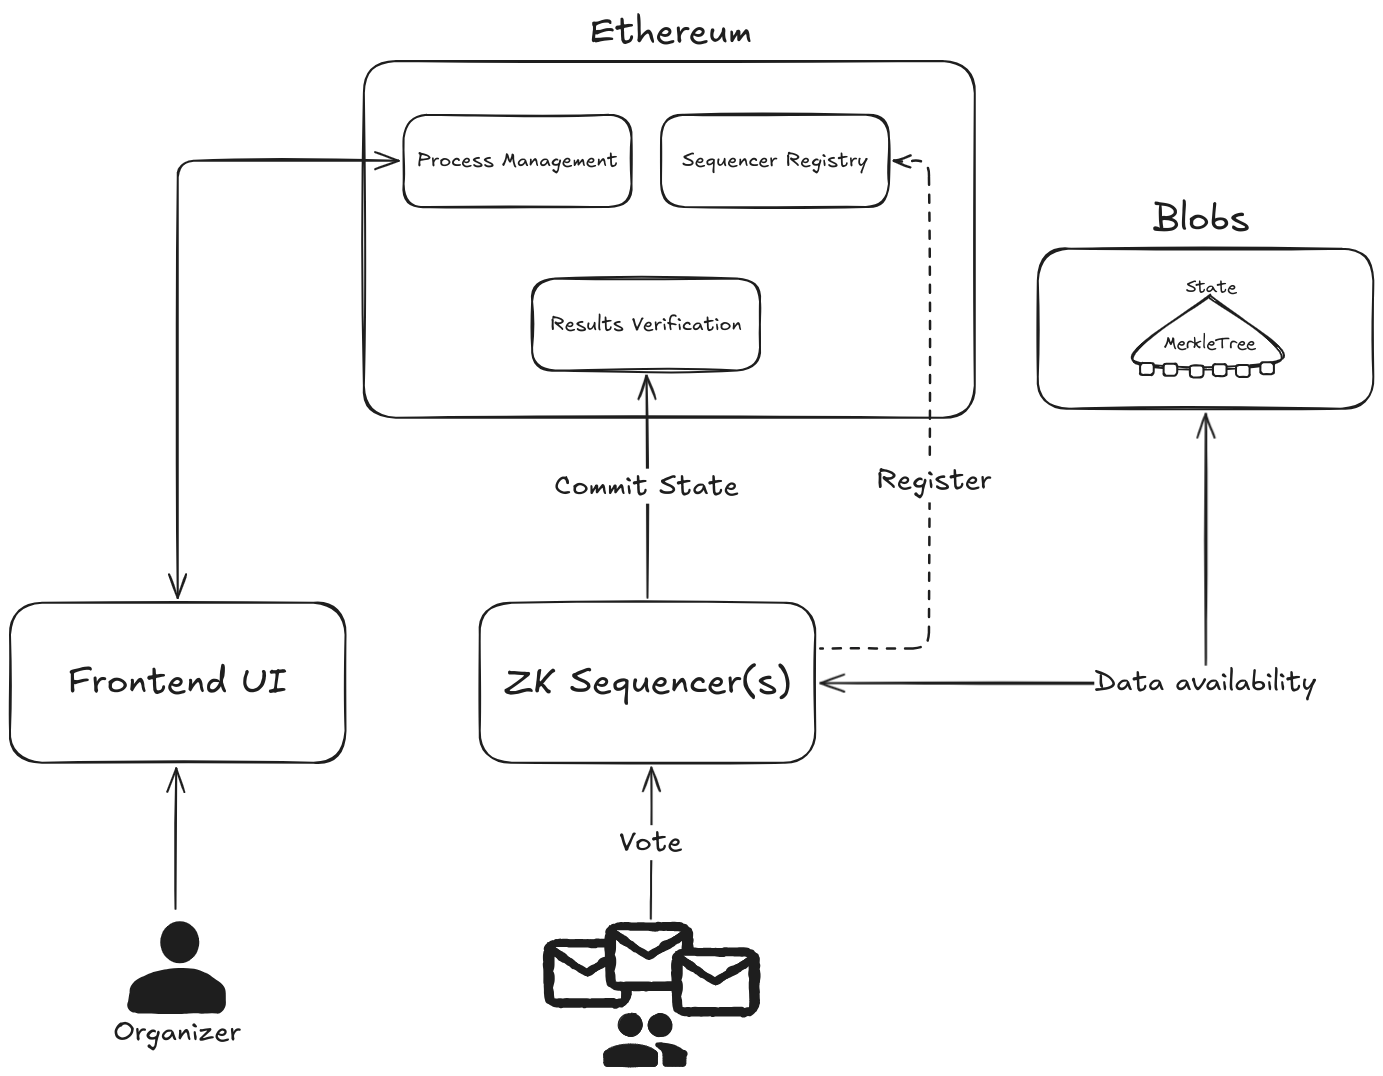
\includegraphics[scale = 0.2, draft = false]{\figs/architecture.png}}
\end{figure}

\subsection{Ethereum}

An Ethereum compatible network is used as the source of truth for the voting system. By leveraging an EVM blockchain, the process management ensures that all transitions are immutable and verifiable by all participants. To this end, we implement several smart contracts.

\begin{itemize}
	\item \textbf{Process Management}: Responsible for the lifecycle management of voting processes. It includes the initiation, monitoring, execution, and closure of voting events.
	
	\item \textbf{Results Verification}: For each voting process, this smart contract maintains the integrity of the cast votes and process lifecycle. It verifies that each state transition committed by a ZK sequencer adheres to the predefined rules.
	
	\item \textbf{Sequencer Registry}: This smart contract keeps track of the existing available sequencers, stores the collateral to ensure good behavior, and it's used to coordinate the distributed key generation when a new Process is created.
\end{itemize}

\subsection{Sequencer}

The Sequencer is a specialized component designed to handle the voting process using zero-knowledge proof mechanisms. It ensures that all transactions related to this process are validated and sequenced. The Sequencers periodically commit the state of the voting process to Ethereum.

\subsection{Frontend User Interface}

The user interface serves as the primary interaction layer for voters and organizers. It provides tools and functionalities needed by organizers to set up, manage, and oversee elections. This interface simplifies the complexities involved in managing a decentralized vote.

\subsection{Data Availability}

For each voting process, the system needs to keep track of the current State Merkle Tree, which contains all information of such processes. A public data availability layer, ensures that all state transitions are available and verifiable and allows the participation of multiple sequencers within the same voting process.

\section{Operation Overview}
\label{sec:operation-overview}
% !TeX root = ../build/main.tex

This chapter provides an overview of the operational workflow of the Vocdoni Z protocol, detailing the sequential phases and roles involved. The process includes the initialization of a voting event, distributed key generation, encrypted vote casting, vote verification, and accumulation, culminating in the publication and public verification of results. Each phase leverages advanced cryptographic techniques to ensure the integrity, privacy, and universal verifiability of the voting process.

\subsection{Simplified Workflow Steps}

\begin{enumerate}
	\item \textbf{Organizer Creates a New Voting Process}
	
		\begin{itemize}
			\item Prepare the census data.
			\item Set voting details such as duration, options, type, etc.
			\item Send the transaction to the Ethereum Process smart contract.
		\end{itemize}
	
	\item \textbf{Sequencers Create the Distributed Threshold Encryption Key}
	
			\begin{itemize}
				\item Use the Sequencer Registry smart contract to coordinate the Distributed Key Generation (DKG).
				\item Provide collateral to ensure correct participation in the DKG.
				\item Download all required data to handle the new vote, such as the census Merkle tree.
			\end{itemize}
	
	\item \textbf{Voting Begins Once the Encryption Public Key (EPK) is Available}
	
	\item \textbf{Voters Cast Their Votes}

			\begin{itemize}
				\item Choose any of the available sequencers.
				\item Fetch their census Merkle proof to prove eligibility.
				\item Use the EPK to encrypt their voting choice.
				\item Generate a zkSNARK to prove the validity of the encrypted vote and adherence to ballot protocol rules.
				\item Send the encrypted vote, Merkle proof, validify proof and identity proof to the sequencer.
			\end{itemize}
	 
	\item \textbf{Sequencers Verify and Accumulate the Votes}

			\begin{itemize}
				\item Fetch Current State: Retrieve the current valid process state root from the Ethereum smart contract and the associated data from Ethereum blobs.
				\item Generate a zkSNARK of state transition, proving: 
						\begin{itemize}
							\item the validity of the zkSNARK proof provided by the voter.
							\item the correct accumulation of votes from users, adding them to the process state.
							\item the correct sum off the new encrypted votes using the homomorphic properties of ElGamal.
							\item the new votes are from eligible users by checking the census Merkle proofs.
							\item the new voters have not already voted by checking their nullifiers, or it is a correct vote overwrite
							\item the data blob hash matches the data used to verify the transition.
						\end{itemize}
				\item Submit Updated State: Send the new state root to the smart contract and store the updated data in Ethereum blobs.
			\end{itemize}
	
	\item \textbf{Smart Contract Verification of the State Transition}

			\begin{itemize}
				\item Verify the zkSNARK proof provided by the sequencer.
				\item Ensure the origin root corresponds to the current stored state root.
				\item Confirm that the blob hash matches the one stored in Ethereum.
			\end{itemize}
	
	\item \textbf{Repeat Until Voting Ends}

			\begin{itemize}
				\item Sequencers accumulate more votes and create state transitions until the finalization of the process.
			\end{itemize}
	
	\item \textbf{Create the Decryption Key}

			\begin{itemize}
				\item Once voting is complete, sequencers publish their shares of the EPK to the Ethereum smart contract.
				\item Decrypt Results: When the threshold of shares is reached, the results can be decrypted by anyone.
				\item Sequencers receive reward for their correct participation depending on the number of sequenced votes.
			\end{itemize}
	
	\item \textbf{Public Verification of the Final Results}
			\begin{itemize}
				\item After the voting period ends and the results are decrypted, anyone can verify the correctness of the final result.
				\item Use the zkSNARK State proof and publicly available data on-chain to ensure the integrity and correctness of the entire voting process.
			\end{itemize} 
\end{enumerate}

\begin{figure}[H]
	\centering
	\fbox{
		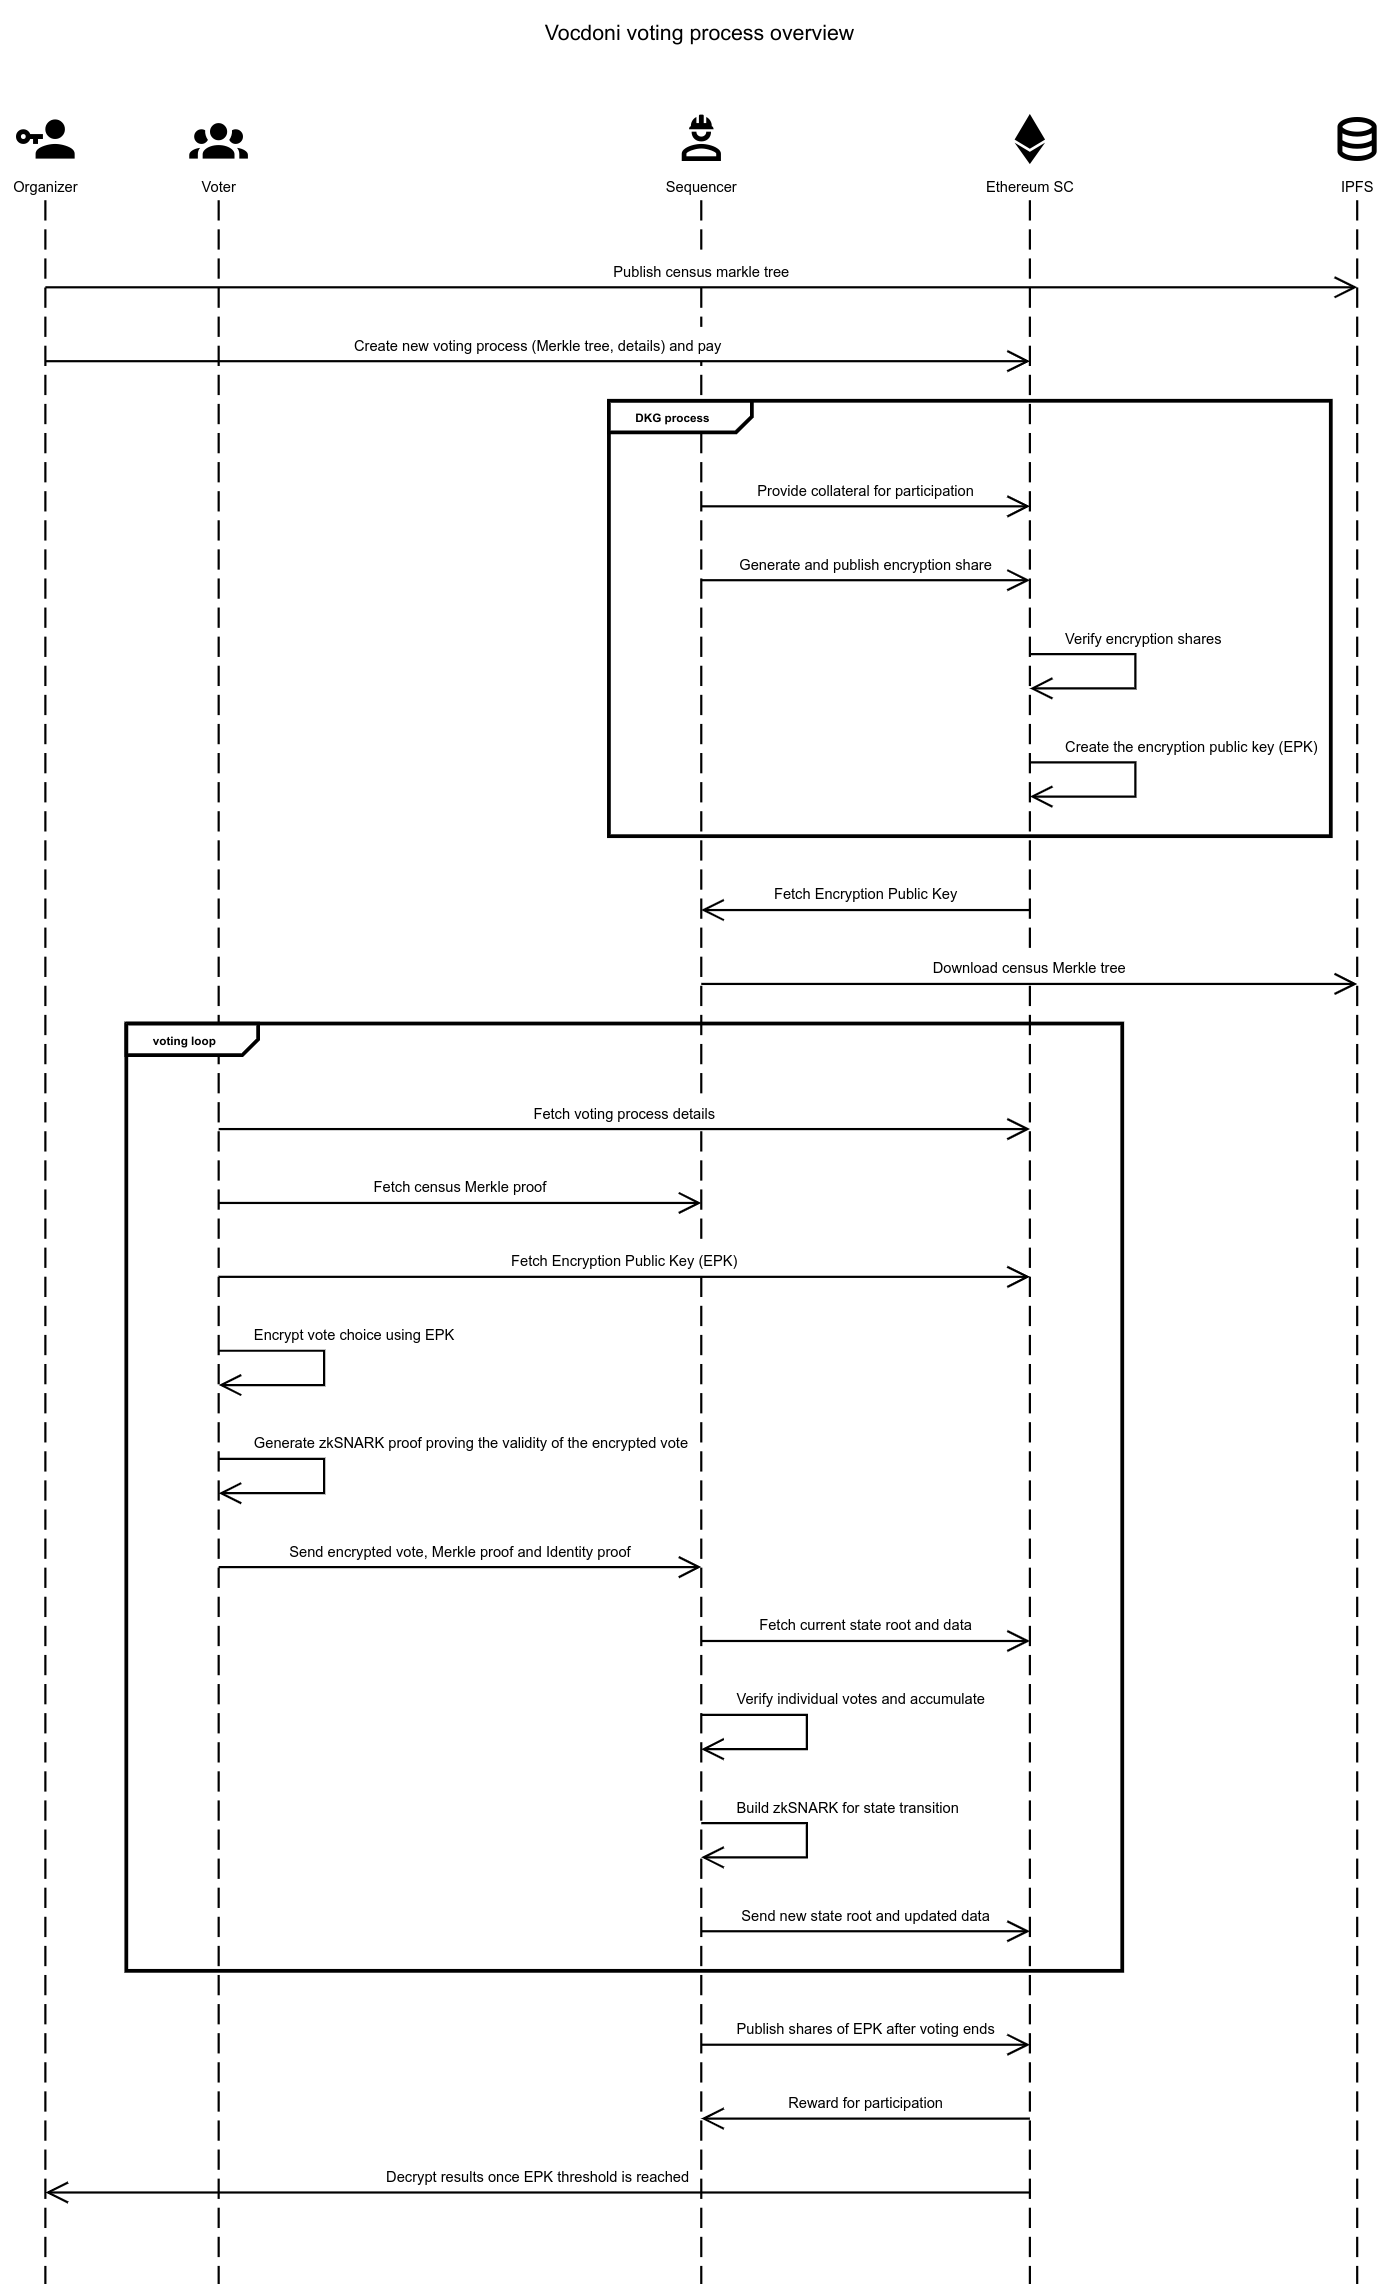
\includegraphics[scale = 0.3, draft = false]{\figs/workflow-simplified.png}}
\end{figure}


\section{Sequencer and State Transitions}
\label{sec:sequencer-state-transition}
% !TeX root = ../build/main.tex

When a new voting process begins, the Sequencer initializes a new State, represented by the root hash of a Merkle tree. This tree encapsulates all essential information about the voting process, including process parameters, voter registry (census), ballot configurations, and initial results.

For each new batch of votes, the Sequencer updates the state by generating a zkSNARK proof that \textbf{validates the state transition from the current Root to a new Root}. This proof is submitted on-chain for settlement. By doing so, we maintain an immutable and verifiable record of the voting process on the blockchain.

This approach allows anyone to access the latest verified state of the voting process from the Results Verification smart contract, along with the necessary data to process subsequent state updates. The system's design enables multiple Sequencers to participate in tallying votes. They can take the current State Root and its associated data to construct the next state, incorporating new votes into the tally. This decentralization of Sequencers helps prevent potential censorship and reinforces the robustness of the voting process.

\subsection{Maintaining the Chain}

The chain of integrity is maintained through a combination of smart contract enforcement and strict zkSNARK circuit constraints. This ensures that each state transition is valid and builds upon the last accepted state without requiring additional mechanisms.

\begin{itemize}
	\item \textbf{Sequential State Roots}: Each state transition updates the Merkle tree from a previous root (`Root1`) to a new root (`Root2`) after processing a batch of votes.
	\item \textbf{Smart Contract Enforcement}: The smart contract verifies that the `Root1` provided in the zkSNARK proof matches the last committed state root stored on-chain. This guarantees that all transitions are sequential and based on the latest accepted state.
	\item \textbf{Proof Validation}: The smart contract uses the zkSNARK verification key to validate the submitted proof. A valid proof confirms that the transition from `Root1` to `Root2` adheres to all protocol rules enforced by the circuit.
	\item \textbf{State Update}: Upon successful verification, the smart contract updates the stored state root hash to`Root2`, ensuring an immutable and continuous chain of states.
\end{itemize}

\subsection{State Merkle Tree Structure}

The State tree contains some special addresses (indices) for storing some required data regarding the voting process:

\begin{itemize}
	\item Address `0x0`: \textbf{Process Identifier}: stores a unique identifier for the voting process.
	\item Address `0x1`: \textbf{Census Root and Type}: contains the information necessary to validate vote proofs.
	\item Address `0x2`: \textbf{Ballot Mode}: encodes rules for validating votes, such as the maximum number of selectable options.
	\item Address `0x3`: \textbf{Threshold Encryption key}: the public key used to encrypt the votes.
	\item Address `0x4`: \textbf{Added Results Accumulator}: stores the aggregated encrypted voting results that need to be added.
	\item Address `0x5`: \textbf{Subtract Results Accumulator}: stores the aggregated encrypted voting results that need to be subtracted.
	\item Any Address: \textbf{Vote addresses}: are stored within the State tree pointing to a voter's identity commitment. Each commitment is a 32-byte hash derived from the voter's unique information and a secret.
	\item Any Address: \textbf{Vote nullifiers}: are stored within the State tree to prevent double voting and to allow vote overwrite. Each nullifier is a 32-byte hash derived from the voter's commitment and a secret.
\end{itemize}

\begin{figure}[H]
	\centering
	\fbox{
		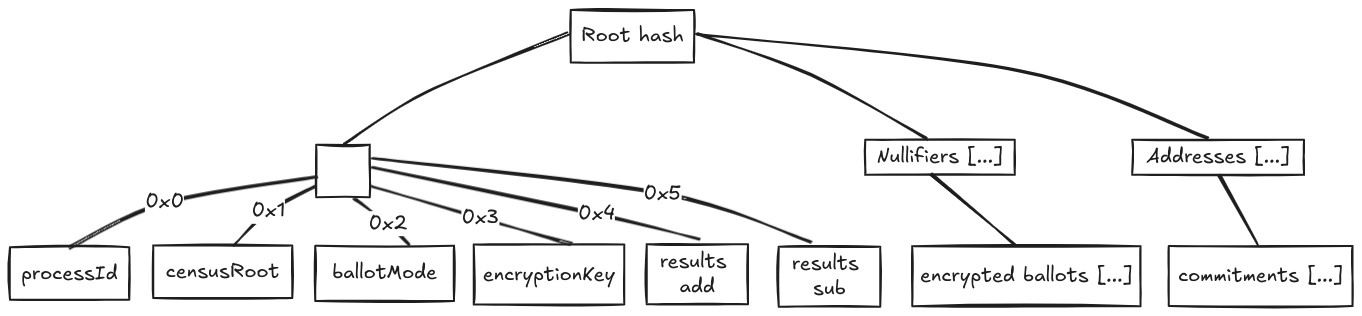
\includegraphics[scale = 0.3, draft = false]{\figs/merkle-tree-state.png}}
\end{figure}

\subsection{The Initial State}

The voting process begins with an initial state where the Merkle Tree Root is established and published on the Process Management smart contract. Predefined parameters are included, but the results are initialized to zero, and no nullifiers are present.

The Process Organizer transaction, contains the initial root and the necessary Merkle proofs. These proofs verify that the initial parameters are correct according to the voting process information and that no additional information is stored. Since the `ProcessId` of the initial state is a unique identifier, there won't be duplicate roots for different processes.

\subsection{State Transition}

To validate and process state transitions, \textbf{we employ a zkSNARK circuit that enforces all protocol constraints}. This circuit proves that the transition from the previous state Root to the new state Root is valid based on the newly processed votes.

\begin{figure}[H]
	\centering
	\fbox{
		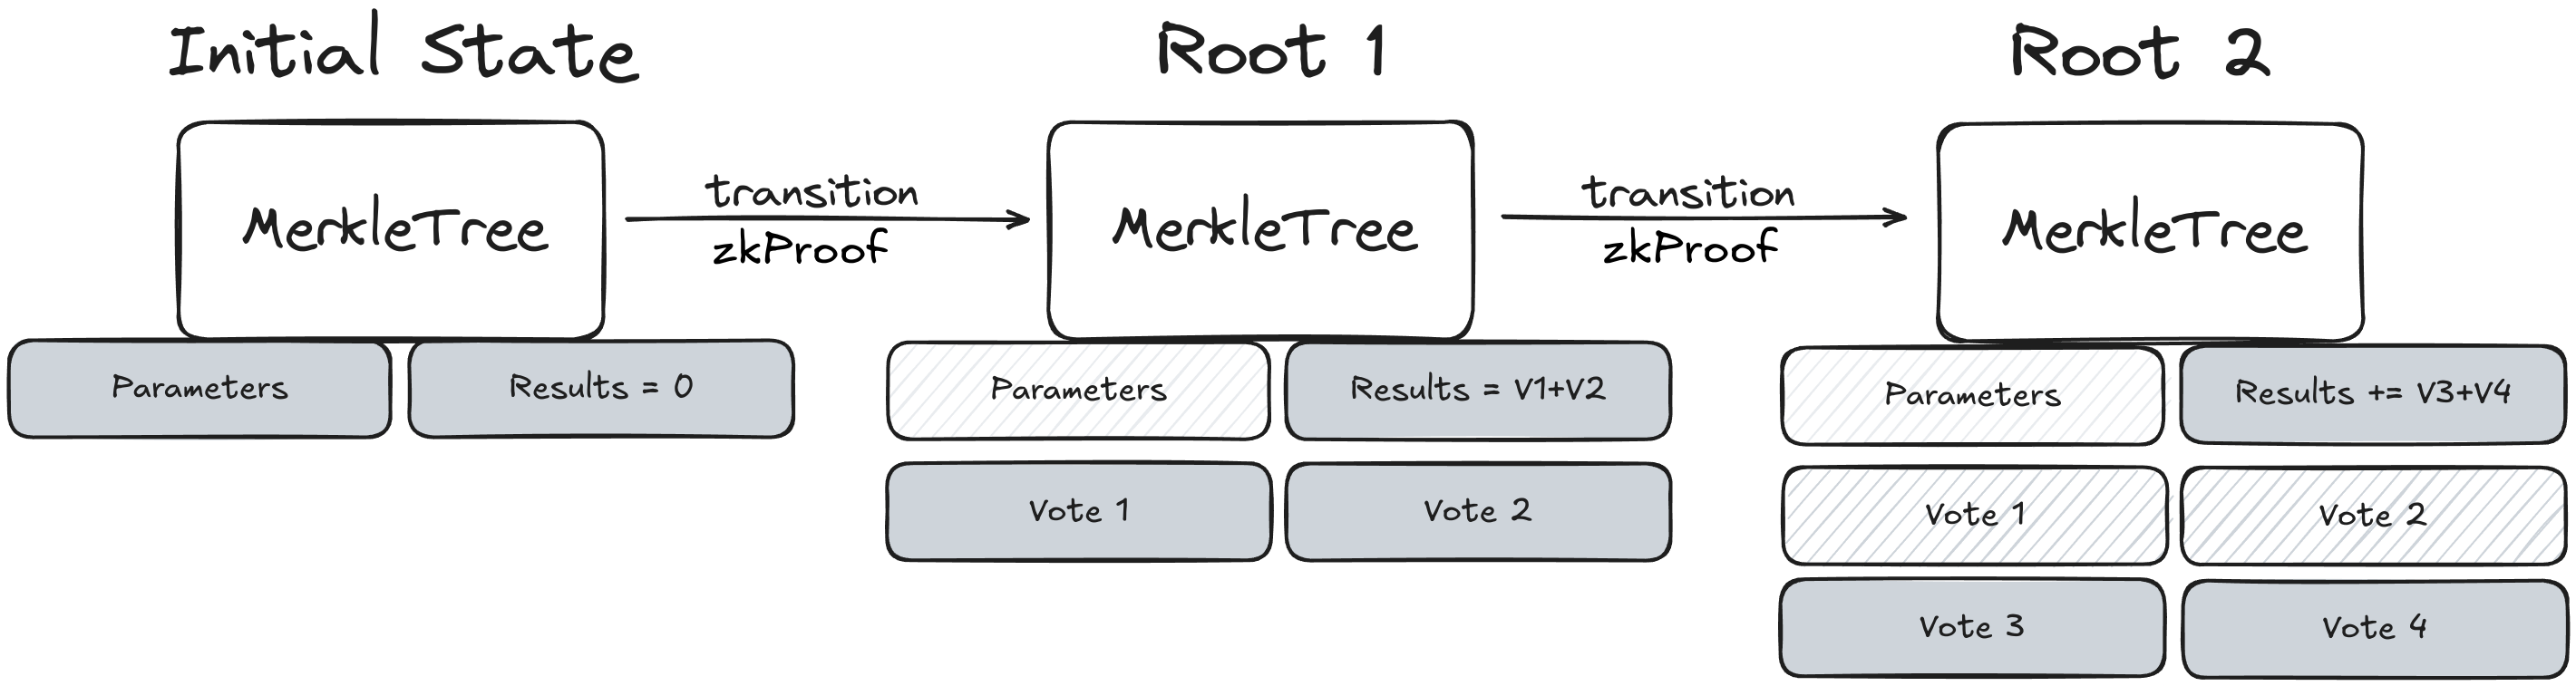
\includegraphics[scale = 0.12, draft = false]{\figs/state-transition.png}}
\end{figure}

The circuit have the following inputs (the public ones are required to verify the proof).

\begin{itemize}
	\item \textbf{Public Inputs:}
			\begin{itemize}
				\item Previous State Root (Root1): The Merkle tree root before the state transition.
				\item New State Root (Root2): The Merkle tree root after the state transition.
				\item Blob Data Commitment (blobCommitment): The commitment to the data blob containing the new votes.
			\end{itemize}
	\item \textbf{Private Inputs:}	
			\begin{itemize}
				\item Votes: The list of new votes being processed, including census proofs and authentication data.
				\item Merkle Proofs of nullifier inclusion: Proofs that each voter nullifier is included in the census.
				\item Merkle Proofs of results update: Proofs that the process results have been correctly updated.
				\item Merkle Tree Update Witnesses: Necessary data (e.g., Merkle paths) to update the Merkle tree from Root1 to Root2.
				\item Process Parameters: Retrieved from Root1 within the circuit.
			\end{itemize}
\end{itemize}

\begin{figure}[H]
	\centering
	\fbox{
		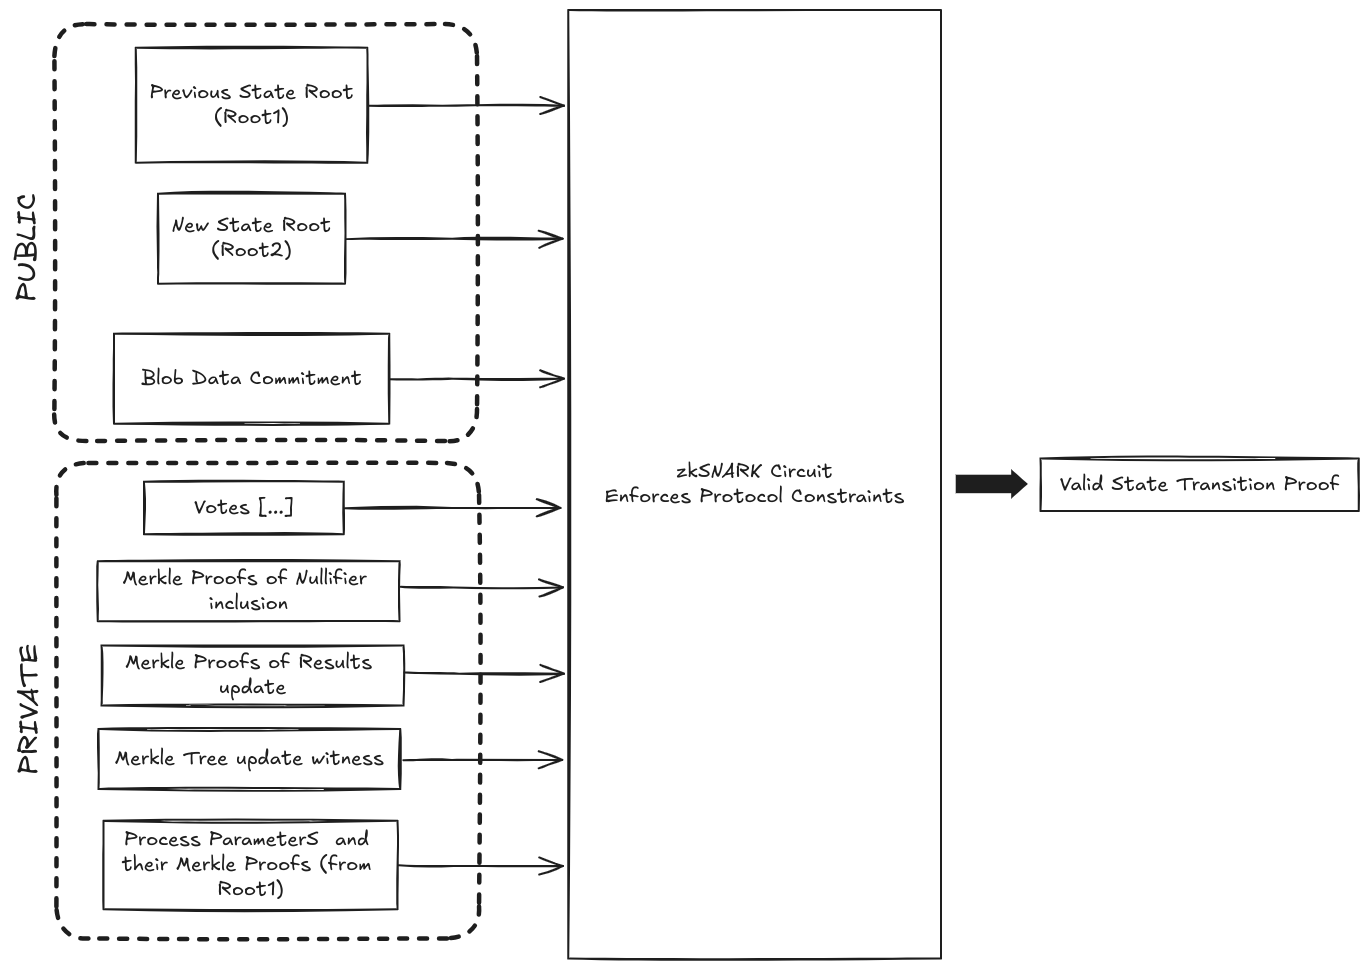
\includegraphics[scale = 0.3, draft = false]{\figs/circuit-inputs.png}}
\end{figure}

The following constraints must be enforced by the circuit.

\begin{itemize}
	\item \textbf{Immutable Process Parameters}: Ensure that critical process parameters (such as `censusRoot` or `processId`) retrieved from `Root1` remain consistent and are not altered in the transition.
	\item \textbf{Vote Validity}: Validate that each vote proof is correct.
	\item \textbf{Voter Eligibility}: Confirm that each voter is included in the census by verifying Merkle proofs of inclusion against the `censusRoot` retrieved from `Root1`.
	\item \textbf{Nullifier Non-Existence}: Ensure that the nullifier for each vote does not exist in the current state (`Root1`), preventing double voting.
	\item \textbf{Nullifier Addition}: Correctly add each new nullifier to the state, resulting in `Root2`, updating the Merkle tree accordingly.
	\item \textbf{Results Update}: Ensure that the voting results are accurately updated by adding the new votes to the previous results retrieved from `Root1`, so that `results2 = results1 + votes`.
	\item \textbf{Blob Data Integrity}: Confirm that the data used in the circuit (votes, nullifiers) corresponds to the `blobCommitment` provided as a public input, ensuring that the votes processed are exactly those published in the data blob.
	\item \textbf{State Transition Validity}: Ensure that the new state root (`Root2`) is correctly computed from `Root1` by applying the validated votes and updates to the Merkle tree.
\end{itemize}

\subsection{Finalization of the Voting Process}

At the conclusion of the voting period, the smart contract ceases to accept new state updates, effectively finalizing the process. The final State is then available on-chain for verification, providing an immutable record of the voting outcome.

\section{The Vote}
\label{sec:vote}
% !TeX root = ../build/main.tex

In the Vocdoni Z system, a vote comprises several components that work together to ensure secure, private, and verifiable voting. These components are:

\begin{enumerate}
	\item Process Identifier
	\item Census Proof
	\item Identity Commitment
	\item Nullifier
	\item Encrypted Ballot and Zero-Knowledge Proof (ZKP)
	\item Signature	
\end{enumerate}

Below, we detail each component and its role in the voting process.

\begin{enumerate}
	\item \textbf{Process Identifier} \\
	
			The \textbf{Process Identifier} (\texttt{ProcessId}) is a unique 32-byte number that uniquely identifies a specific voting process within the Vocdoni Z ecosystem. It encapsulates essential information, including the rules and constraints for ballots and the unique identifier of the Vocdoni Z blockchain instance.\\
			
	\item \textbf{Census Proof} \\
			
			The \textbf{Census Proof} serves as the voter's identity verification mechanism, ensuring that only eligible voters can participate. Depending on the process configuration, the voter provides:
			\begin{itemize}
				\item \textbf{Merkle Tree-Based Proof}: A Merkle proof showing inclusion in the census.
				\item \textbf{Credential Service Provider (CSP)}: A credential issued by a trusted third party. \\
			\end{itemize}
			
	\item \textbf{Identity Commitment}\\
	
			The \textbf{Commitment} $C$ is used to prevent a voter from registering multiple nullifiers and to avoid collisions if different voters choose the same secret.
			
			$$ C = \text{Hash} (\text{Address} || ProcessId || s). $$
			
			\begin{itemize}
				\item \textbf{Stored in State Merkle Tree (SMT)}: Indexed by the voter's address.
				\item \textbf{Prevents Multiple Registrations}: Each address can have only one commitment, ensuring a voter cannot register multiple secrets.
				\item \textbf{Collision Resistance}: Including the address in $C$ ensures that commitments are unique even if voters choose the same secret $s$.
			\end{itemize}
			
			The secret $s$ can be implemented from different ways or a combination of them, such as:
			
			\begin{itemize}
				\item A secure enough Password introduced by the user.
				\item A signature of a specific text.
				\item A random input that the user must store to allow potential vote overwrite.\\
			\end{itemize}
	
	\item \textbf{Nullifier} \\
	
			The \textbf{Nullifier} $N$ is a 32-byte hash used to:
			
			\begin{itemize}
				\item \textbf{Prevent Double Voting}: Ensures each voter can cast only one vote or overwrite their previous vote.
				\item \textbf{Allow Vote Overwriting}: Voters can submit a new vote with the same nullifier to replace their previous vote.
				\item \textbf{Provide Anonymity}: Cannot be linked back to the voter's identity without knowledge of the secret $s$.
			\end{itemize}
		
			$$ N = \text{Hash}(\text{C} || s) $$ 
			
	\item \textbf{Encrypted Ballot and Zero-Knowledge Proof (ZKP)} \\
	
			The ballot contains the voter's selections encoded according to the ballot protocol rules. To ensure privacy, the ballot is encrypted using the ElGamal cryptosystem over elliptic curves, which allows homomorphic combination of encrypted votes.
			
			\textbf{Encryption process}:
			
			\begin{itemize}
				\item The voter's choice $m$ is encoded as a point on the elliptic curve.
				\item The voter selects a random scalar $k \in [1, n-1]$, where is the order of the elliptic curve group.
				\item Compute the ciphertext components:
					\begin{itemize}
						\item $C_1 = k \cdot G$
						\item $C_2 = M + k \cdot H$
					\end{itemize}
				\item The ciphertext is the pair $(C_1, C_2)$.
			\end{itemize}


			\textbf{Zero-Knowledge Proof (ZKP)}:
			
			The voter generates a ZKP to prove the correctness of the ballot and encryption process:
			
			\begin{enumerate}
				\item \textbf{Correctness of Encryption}: Ensures the ciphertext $(C_1, C_2)$ is correctly computed from the plaintext message $M$ and random scalar $k$.
				\item \textbf{Compliance with Ballot Protocol Rules}: The plaintext vote adheres to the ballot protocol constraints, such as valid choices and allowed number of selections.
				\item \textbf{Correct Computation of Commitment and Nullifier}:
						\begin{itemize}
							\item \textbf{Commitment}: $C = \text{Hash} (\text{Address} || ProcessId || s).$
							\item \textbf{Nullifier}: $N = \text{Hash}(\text{C} || s)$.
							\item The voter knows the secret linking the commitment and nullifier.
						\end{itemize}
			\end{enumerate}
		
			\textbf{Inputs to the ZKP Circuit}:
			
			\begin{itemize}
				\item \textbf{Public Inputs}:
						\begin{itemize}
							\item Encrypted Ballot $(C_1, C_2)$.
							\item Ballot Protocol Configuration.
							\item Encryption Parameters.
							\item Voter's Weight
							\item Commitment $C$.
							\item Nullifier $N$.
						\end{itemize}
				\item \textbf{Private Inputs}:
						\begin{itemize}
							\item Plaintext Vote $m$.
							\item Secret $s$.
							\item Random Scalar $k$.
							\item Voter's Address (used internally in the computation of $C$).
						\end{itemize}
			\end{itemize}
		
	\begin{figure}[H]
		\centering
		\fbox{
			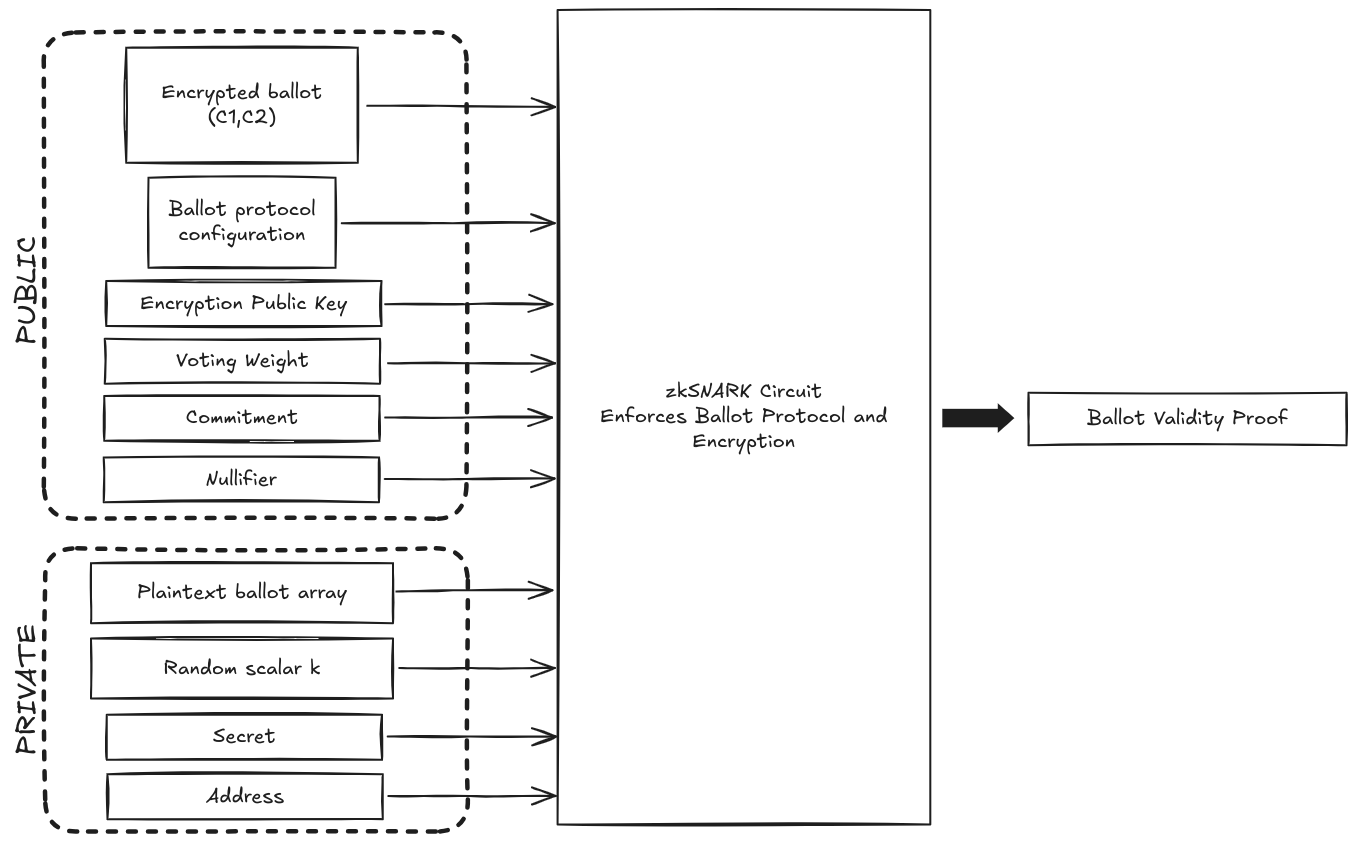
\includegraphics[scale = 0.3, draft = false]{\figs/vote-circuit-inputs.png}}
	\end{figure}
		
	
	\item \textbf{Signature}\\
	
			The \textbf{Signature} authenticates the vote and ensures that it was cast by a legitimate voter. The voter signs necessary components using their private key, depending on the census configuration (e.g., ECDSA, EdDSA, RSA).	
\end{enumerate}


\section{The Ballot Protocol}
\label{sec:ballot-protocol}
% !TeX root = ../build/main.tex

\martai{All this section is the original old text.}

The \textit{Vocdoni ballot protocol} is a simple and efficient mechanism for casting and tallying votes in any type of election or collective decision-making process. Each voting process consists of one or several fields and voters are required to provide a response for each of these fields in their ballot.

The responses in the ballot are represented as a sequence of natural numbers, each corresponding to the voter’s choice for the respective field. Results are accumulated into a single array. Each position in the array corresponds to the sum of all votes cast for that field across all voters.

The ballot protocol is defined by a set of configurable variables that dictate how votes must be cast. This way the protocol can accommodate a wide range of voting processes and behaviors.

\begin{enumerate}
	\item \maxcount: Defines the maximum number of fields in a ballot (max 64).
	\item \maxvalue: The maximum allowable value for any field in a ballot (if greater than 0).
	\item \minvalue: The minimum allowable value for any field in a ballot (default 0).
	\item \uniquevalues: Specifies whether voters can select the same value multiple times within a ballot (default false).
	\item \maxtotalcost: Limits the sum of all field values in a ballot (if greater than 0).
	\item \mintotalcost: Specifies a minimum required total sum of field values in a ballot (default 0)
	\item \costexponent: Defines the exponent used to calculate the "cost" of votes for each field (default 1
\end{enumerate}

\begin{figure}[H]
	\centering
	\fbox{
		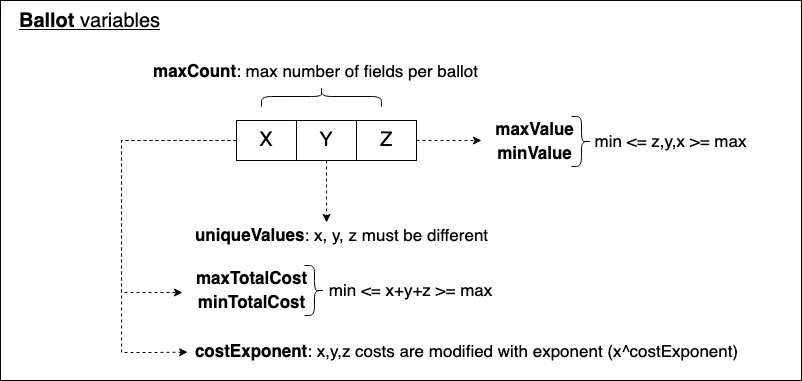
\includegraphics[scale = 0.4, draft = false]{\figs/ballot-variables.png}}
\end{figure}

\paragraph{Example 1: Rating candidates.}

Consider a voting process where voters are asked to rate three candidates: Lennon, Hendrix, and Joplin. Voters rate each candidate from 0 to 5 stars, and each vote is represented as an array where each position corresponds to the candidate’s rating. The configuration of this voting would be the following:

\begin{itemize}
	\item \maxcount: 3
	\item \maxvalue: 5
	\item \uniquevalues: Yes
\end{itemize}

Ballots:

\begin{itemize}
	\item Vote 1: \texttt{[3, 2, 5]} (3 stars for Lennon, 2 stars for Hendrix, 5 stars for Joplin)
	\item Vote 2: \texttt{[4, 3, 2]}
	\item Vote 3: \texttt{[2, 4, 5]}
\end{itemize}

After accumulating the votes:

\begin{itemize}
	\item Results Array: \texttt{[3+4+2, 2+3+4, 5+2+5] = [9, 9, 12]}\\
	Lennon received 9 points, Hendrix received 9 points, and Joplin received 12 points.
\end{itemize}

\paragraph{Example 2: Quadratic voting for resource allocation.} 

In a scenario where voters distribute a fixed number of credits across different options (e.g., selecting funding levels for NGOs), the ballot allows voters to assign multiple points, but the cost of casting multiple votes for a single option increases quadratically.

Configuration:

\begin{itemize}
	\item \maxcount: 4
	\item \maxtotalcost: 12 (credits)
	\item \costexponent: 2 (quadratic)
\end{itemize}

Ballots:

\begin{itemize}
	\item Vote 1: \texttt{[2, 2, 2, 0]}
	\item Vote 2: \texttt{[1, 1, 3, 1]}
	\item Vote 3: \texttt{[0, 2, 1, 2]}
\end{itemize}


After accumulating the votes:


\begin{itemize}
	\item Results Array: \texttt{[2+1+0, 2+1+2, 2+3+1, 0+1+2] = [3, 5, 6, 3]} \\
	Each position in the array represents the total sum of credits allocated to each NGO.
\end{itemize}

\martai{Cost may be dependant on the voter's weight.}

\section{The voting encryption key}
\label{sec:voting-encryption-key}
% !TeX root = ../build/main.tex

In the Vocdoni Z system, the privacy of the voting process is ensured through the use of a \textbf{Threshold Homomorphic Encryption Scheme}. Specifically, the \textbf{Threshold ElGamal Cryptosystem over elliptic curves} is used. This cryptosystem provides both homomorphic and threshold properties essential for secure and verifiable digital voting.

Encrypted messages can be combined to produce an encryption of the sum of the original plaintexts without decrypting them. In the context of voting, this allows for the secure aggregation of votes while keeping the voter's choice private.

\begin{enumerate}
	\item \textbf{Collaborative Key Generation:} 
			\begin{itemize}
				\item The public key is generated collaboratively among the sequencers without any single party knowing the entire private key.
				\item Utilizes a \textbf{Distributed Key Generation (DKG)} protocol to share the private key $s$ among $n$ sequencers using a threshold scheme.
			\end{itemize}
	\item \textbf{Encryption}: Given a message $m$ encoded as a point $M(M = mG)$ on the elliptic curve:
		\begin{itemize}
			\item Select a random scalar $k \in [1, n-1]$ and consider $H = sG$.
			\item Compute:
				\begin{itemize}
					\item $C_1 = k\cdot G$
					\item $C_2 = M + k \cdot H$
				\end{itemize}
			\item The ciphertext is $(C_1, C_2)$.
		\end{itemize}

	\item \textbf{Homomorphic Addition}: The ElGamal cryptosystem over elliptic curves supports additive homomorphism for messages represented as points:
		\begin{itemize}
			\item Given two ciphertexts $(C_1^{(1)}, C_2^{(1)})$ and $(C_1^{(2)}, C_2^{(2)})$, their component-wise addition yields:
				\begin{itemize}
					\item $C_1^{\text{sum}} = C_1^{(1)} + C_1^{(2)}$
					\item $C_2^{\text{sum}} = C_2^{(1)} + C_2^{(2)}$
				\end{itemize}
			\item The aggregated ciphertext decrypts to the sum of the messages:
				\begin{itemize}
					\item $M^{\text{sum}} = M_1 + M_2$
				\end{itemize}
		\end{itemize}
	
	\item \textbf{Decryption}:
	
			\begin{itemize}
				\item To decrypt an aggregated ciphertext (total sum of votes), a minimum number of sequencers (the threshold ) must provide their partial decryption shares. Each Sequencer compute $D_i = s_i \cdot C_1$
				\item \textbf{Combine Partial Decryptions}:
					\begin{itemize}
						\item Use Lagrange interpolation to combine the $D_i$ and recover $s\cdot C_1$.
						\item Substract from $_c2$ to obtain the aggregated message point:
							\begin{itemize}
								\item $M^{\text{sum}} = C_2 + s \cdot C_1$
							\end{itemize}
						\item Extract the message $m$ from $M$ by solving the discrete logarithm:
							\begin{itemize}
								\item $m = \log_G M$
							\end{itemize}
					\end{itemize}
			\end{itemize}
		
	For solving the discrete logarithm problem and compute the final results, since the message is small, it can be done via brute-force search or using the algorithm \textbf{baby-step giant-step}.

\end{enumerate}

\section{The distributed key generation (DKG)}
\label{sec:distributed-key-generation}
% !TeX root = ../build/main.tex

Vocdoni Z employs a Distributed Key Generation (DKG) protocol that allows a group of participants (Sequencers) to jointly generate a public/private key pair for the ElGamal cryptosystem without any single participant knowing the complete private key. Instead, each participant holds a share of the private key, and only a threshold number of participants can collaborate to decrypt messages (the threshold is configurable). This enhances security by eliminating the need for a trusted dealer and protecting against single-point failures.

\subsection{Properties}

\begin{itemize}
	\item \textbf{Decentralized Key Generation}: No single party knows the complete secret key.
	\item \textbf{Coordinated via Ethereum}: The parties do not need to interact directly, they use an Ethereum Smart Contract to bootstrap the process and exchange the required information.
	\item \textbf{Threshold Security}: A minimum number of participants (threshold) is required to reconstruct the secret.
	\item \textbf{Verifiable Shares}: Parties and Ethereum can verify the correctness of the shares they receive.
	\item \textbf{Scalability}: Supports any number of participants and configurable threshold.
\end{itemize}

\subsection{Protocol Steps}

\begin{enumerate}
	\item \textbf{Initialization}:
			\begin{itemize}
				\item The Ethereum Smart Contract provides the initial parameters:
						\begin{itemize}
							\item \textbf{Threshold} $t$: Minimum number of participants required to decrypt messages.
							\item \textbf{Total Participants} $n$: : Total number of sequencers involved.
							\item \textbf{Elliptic Curve Parameters}: Choose a suitable elliptic curve with generator point $G$ and order $q$.
						\end{itemize}
			\end{itemize}
	\item \textbf{Secret Polynomial Generation}:
			\begin{itemize}
				\item Each participant $P_i$ generates a random secret polynomial of degree $t-1$:
						$$f_i (x) = a_{i,0} + a_{i, 1}x + a_{i,2}x^2 + \dots + a_{i, t-1}x^{t-1}$$
						\begin{itemize}
							\item Coefficients $a_{i,j} \in \mathbb{Z}_q$ are randomly selected.
							\item The constant term $a{i,0}$ is $P_i$'s individual secret.
						\end{itemize}
			\end{itemize}
	\item \textbf{Commitment to Coefficients}:
			\begin{itemize}
				\item Participants compute public commitments to their polynomial coefficients: $C_{i,j} = a_{i,j}\cdot G$
					\begin{itemize}
						\item These commitments are points on the elliptic curve and are published to all participants.
						\item This ensures transparency and allows others to verify shares without revealing secrets.
					\end{itemize}
			\end{itemize}
	\item \textbf{Share Computation}:
			\begin{itemize}
				\item Each participant computes shares for every other participant  $P_j$: $s_{i,j} = f_i(j)$
					\begin{itemize}
						\item The shares $s_{i,j} \in \mathbb{Z}_q$ are secret scalar values.
					\end{itemize}
			\end{itemize}
	\item \textbf{Secure and Verified Distribution}:
			\begin{itemize}
				\item Shares are encrypted before distribution using a simplified version of the \textbf{Elliptic Curve Integrated Encryption Scheme (ECIES)}, since we only need to encrypt a scalar:
				\item Each participant provides a zkSNARK proof to prove:
					\begin{itemize}
						\item The correctness of the encrypted share.
						\item Compliance with the DKG protocol rules.
					\end{itemize}
				\item This allows the smart contract on Ethereum to verify the validity without revealing secrets.
			\end{itemize}
	\item \textbf{Aggregation of Shares}:
			\begin{itemize}
				\item Each participant computes their private key share by summing the shares received (including their own): $s_j = \sum_{i ^1}^ns_{i,j} \mod q$
				\item This becomes $P_j$'s portion of the collective private key.
			\end{itemize}
	\item \textbf{Public Key Computation}:
			\begin{itemize}
				\item Participants compute the collective public key: $PK = \sum_{i = 1}^n C_{i,0}$
					\begin{itemize}
						\item Since $C_{i,0} = a_{i,0}\cdot G$, the public key is effectively: $PK = s\cdot G$ where $s = \sum_{i = 1}^n a_{i,0} \mod q$ is the collective private key (unknown to any single participant).
					\end{itemize}
			\end{itemize}
	\item \textbf{Public Key Distribution}:
			\begin{itemize}
				\item Any of the participants can publish the collective public key $PK$ to the Ethereum smart contract.
			\end{itemize}
\end{enumerate}

\section{Receipt-Freeness}
\label{sec:receipt-freeness}
% !TeX root = ../build/main.tex

In democratic processes, the ability of voters to cast their votes freely, without undue influence or coercion, is crucial. A critical aspect of maintaining this freedom is ensuring receipt-freeness, preventing voters from being able to prove to third parties how they voted. Vocdoni Z implements receipt-freeness by leveraging the properties of the ElGamal cryptosystem, and zkSNARKs.

\subsection{Ballor re-encryption}

The ElGamal cryptosystem over elliptic curves supports additive homomorphism, allowing operations to be performed on ciphertexts that translate to addition on the underlying plaintexts. Re-encryption is a process that refreshes the randomness of a ciphertext without changing the underlying plaintext message. This makes computationally infeasible to link the original and re-encrypted ciphertexts.

\subsection{Handling Receipts}

To prevent voters from being able to prove how they voted, Vocdoni Z employs re-encryption of ballots by the Sequencers. When a voter submits an encrypted ballot, the Sequencer re-encrypts it before storing it in the state Merkle tree.

This way, the system ensures that voters cannot produce a receipt of their vote by revealing r since the stored ciphertext no longer corresponds to r. This prevents vote-buying and coercion by third parties.

\subsection{Handling Collusion}

To further enhance receipt-freeness and mitigate the risk of collusion between voters and Sequencers, Vocdoni Z allows voters to overwrite their votes. A voter can submit multiple votes, with each new submission replacing the previous one.

When a Sequencer receives a new vote from a voter who has already voted, it performs the following steps:

\begin{enumerate}
	\item \textbf{Detect Overwrite}: The Sequencer checks the state Merkle tree using the voter's nullifier to determine if the voter has previously cast a vote.
	\item \textbf{Subtract Previous Vote}: The Sequencer takes the existing encrypted ballot and adds it to a "Subtractive Results" accumulator. This effectively negates the previous vote in the final tally.
	\item \textbf{Add New Vote}: The new encrypted ballot is added to the "Results" accumulator.
	\item \textbf{Update State Merkle Tree}: The Sequencer re-encrypts the new ballot and updates the state Merkle tree with this re-encrypted ballot.
\end{enumerate}

\subsection{Concealing Vote Overwrites}

To prevent observers from detecting when overwrites occur, the Sequencers regularly re-encrypt a random subset of ballots in the state Merkle tree during each state update. This process obscures the occurrence of overwrites, as re-encryptions are indistinguishable from standard re-randomizations performed for privacy enhancement.

By re-encrypting random ballots, the system increases the entropy and makes it statistically improbable for an adversary to determine if a specific ballot was overwritten or simply re-randomized.

\section{How User's Privacy Is Preserved}
\label{sec:user-privacy-preserving}
% !TeX root = ../build/main.tex

Vocdoni Z ensures user anonymity by anonymizing both the ballot and the voter's identity, employing cryptographic techniques that maintain privacy even in the face of future quantum computing threats. The system uses the \textbf{ElGamal Homomorphic Encryption scheme} to encrypt ballots, allowing for the aggregation of votes without revealing individual choices. Since encrypted ballots are stored in public repositories like Ethereum blobs—which, although removed after some weeks, may still be accessible—it is crucial to prevent any association between decrypted ballots and voter identities. By decoupling the voter's identity from their encrypted ballot through the use of secrets and cryptographic hashes, even if an adversary decrypts the ballots in the future, they cannot link them back to individual voters.

The identity anonymization acts as a \textbf{double security factor}, enhancing long-term privacy. While the Sequencer processing the vote can identify the voter (since voters submit proofs of eligibility and commitments), there is no incentive for the Sequencer to make this information public, and the Sequencer cannot decrypt the voter's ballot because they do not possess the private decryption keys. This ensures that voter choices remain confidential.

We have adopted this partial identity anonymization because generating fully anonymous proofs using zkSNARKs directly from digital signatures (e.g., ECDSA/EdDSA or RSA) is computationally intensive for client-side devices like browsers and smartphones. Our priority is to support a wide range of devices, making the system accessible to as many voters as possible. In the future, as cryptographic technology advances and client devices become more powerful, we anticipate being able to generate such zero-knowledge proofs efficiently on the client side. This would enable us to fully anonymize the client's identity in addition to the ballot, further enhancing user privacy without compromising accessibility or user experience.

\section{Quantum Resistance}
\label{sec:quantum-resistance}
% !TeX root = ../build/main.tex

As quantum computing technology advances, it poses significant challenges to classical cryptographic schemes that underpin the security of digital systems, including voting platforms like Vocdoni Z. Ensuring that the system remains secure in the face of quantum threats is crucial for its longevity and trustworthiness.

Quantum computers have the potential to solve certain mathematical problems exponentially faster than classical computers. Notably, Shor's algorithm allows quantum computers to efficiently factor large integers and compute discrete logarithms, undermining the security of widely used cryptographic schemes such as RSA, DSA, ECDSA, and the ElGamal cryptosystem.

However, the design of Vocdoni Z incorporates mechanisms that preserve voter anonymity even in the face of future quantum attacks:

\begin{itemize}
	\item \textbf{Detachment of Identity and Encrypted Ballot}: The voter's identity and their encrypted ballot are decoupled through the use of a secret in the nullifier. The nullifier is computed as:
		$$ N = \text{Hash}(\text{ProcessId} || s) $$	
	where is a secret known only to the voter. This means that even if an adversary decrypts the encrypted ballots using a quantum computer, they cannot link a decrypted vote back to a voter's identity in the census without knowledge of the secret $s$.
	\item \textbf{Quantum-Resistant Hash Functions}: The \textbf{Nullifier} and \textbf{Commitment} are computed using cryptographic hash functions that are believed to be resistant to quantum attacks (e.g., SHA-3). While Grover's algorithm can provide a quadratic speedup in searching for preimages, using sufficiently long hash outputs (e.g., 256 bits) mitigates this risk.
\end{itemize}

To further safeguard against quantum threats, the following measures can be implemented in the futre:

\begin{enumerate}
	\item Adopt post-quantum signature schemes. Replace ECDSA/EdDSA with quantum-resistant algorithms such as \textbf{CRYSTALS-Dilithium}, \textbf{Falcon}, or \textbf{Rainbow}, which are based on hard lattice problems.
	
	\item Explore lattice-based homomorphic encryption schemes. Replace ElGamal cryptosystem with quantum-resistant alternatives such as the \textbf{Brakerski-Gentry-Vaikuntanathan (BGV)} scheme or the \textbf{Brakerski/Fan-Vercauteren (BFV)}.
	
	\item Adopt quantum-resistant zero-knowledge proof systems, such as zkSNARK constructions based on post-quantum assumptions or \textbf{zkSTARKs}.
\end{enumerate}

\section{The Vocdoni Token (VOC)}
\label{sec:vocdoni-token}
% !TeX root = ../build/main.tex

Vocdoni Z introduces the Vocdoni token (VOC) as a key element of its decentralized voting ecosystem, playing a crucial role in the protocol's sustainability.
The token serves multiple utility functions that align the incentives of all participants (voting organizers, sequencers, and voters) ensuring the integrity, efficiency, and security of the voting system.

\subsection{Roles of the VOC}

\begin{enumerate}
	\item \textbf{Collateral for Sequencers}: Sequencers are required to stake VOC tokens as a collateral to participate in the protocol. This serves as a safeguard to ensure responsible participation. If a sequencer behaves improperly (whether due to malicious intent or unintentional errors) it can face penalties, including the loss of part of its staked tokens.
	\item \textbf{Incentive Mechanism}: Sequencers earn rewards in VOC tokens based on their contribution to processing valid votes and maintaining the network. Rewards are proportional to the number of valid votes successfully added to the shared state.
	\item \textbf{Payment for Voting Processes}: Voting processes organizers use VOC tokens to cover the costs of creating and managing voting processes. The costs depend on factors like the size of the voting registry, the voting period's duration, and the desired level of security (based on the number of participating sequencers).
	\item \textbf{Governance}: The VOC token facilitates decentralized governance by giving the token holders the right to participate in the project governance. Token holders can influence on important matters such as protocol upgrades, ecosystem development, and other initiatives aimed to enhance various aspects of Vocdoni Z. This ensures that the project evolves in a transparent, community-driven manner.
\end{enumerate}

\subsection{Economics for Organizers}

Organizers of voting processes pay fees in VOC tokens to create and manage their voting events. These fees cover operational costs and incentivize the sequencers.

The costs of voting processes vary based on the following factors:

\begin{itemize}
	\item \textbf{Maximum Number of Votes}: Larger voter registries require more resources for processing.
	\item \textbf{Voting Duration}: Longer voting periods demand extended resource commitments from sequencers.
	\item \textbf{Security Level}: Organizers can adjust the number of participating sequencers to balance between cost and security needs.
\end{itemize}

Fees must be paid upfront but can be partially reimbursed. The formula for calculating the reimbursement is:

$$ \text{Reimbursement} = \text{TotalCost} - \text{TotalReward} - \text{BaseCost} $$

Given that there is a list of eligible voters for each voting process, organizers should reserve space equal to the maximum number of voters, anticipating that all eligible voters may participate. However, since this is unlikely, a portion of the reward pool may be reimbursed.

The components of this formula are defined in the following sections.

\subsection{Voting process cost model}

The process cost model defines how the cost for a given process is calculated.
Considering sequencer-specific capacities, process duration, number of voters and security costs, we define following components formula:

$$ \text{totalCost} = \text{baseCost} + \text{capacityCost} + \text{durationCost} + \text{securityCost} $$

\subsubsection{Components definition}

\begin{itemize}
	\item \textit{baseCost}: The base cost is a fixed fee charged by the sequencer to set up a voting process based on a fixed value plus the number of and a fixed factor. It is independent of the process duration, or the security level. This part cannot be reimbursed thus is a portion of the that will alwways be rewarded to the sequencers.
		$$ baseCost = fixedCost + maxVotes \cdot p $$
		Where:
		\begin{itemize}
			\item $fixedCost$ is a fixed base fee defined into the protocol.
			\item $maxVotes$ is the maximum number of votes of a given voting process.
			\item $p$ is a small lineal factor defined into the protocol.
		\end{itemize}
	
	\item $capacityCost$: It defines the cost given the current occupancy of the sequencer network. This component models the cost of reserving space for voting processes, relative to the number of sequencers available, the number of running voting processes and the maximum numbers of voters. The cost increases non-linearly as the number available sequencers approaches to the total number of sequencers and the number of running voting processes grows, so when there are fewer sequencers available and big number of voting processes running, the capacity becomes more valuable.
		$$
		k_1 \cdot \left( \frac{\text{totalVotingProcesses}}{totalSequencers - usedSequencers + \epsilon} \cdot maxVotes \right)^a
		$$ 
		\begin{itemize}
			\item $k_1$: A scaling factor controlling the impact of sequencers usage.
			\item $totalVotingProcesses$: The total number of running voting processes.
			\item $totalSequencers$: The total number of registered sequencers.
			\item $usedSequencers$: The number of sequencers that are already handling other voting processes.
			\item $a$: An exponent that controls how sharply the cost increases as the used capacity approaches the total available capacity. In other words, it controls the non-linearity of the cost increase.
			\item $\epsilon$: Is a very small number that avoids zero division.
		\end{itemize}
	
	\item $durationCost$: This component models the cost of running the process for a specific duration, where longer processess incur more cost. The scaling is non-linear, meaning that shorter processes are more cost-efficient, while longer processes are increasingly expensive.
	
		It is expected to have a minimum and maximum duration thresholds (e.g 1 hour to 1 year).
	
		$$ k_2 \cdot processDuration^b $$
		
		\begin{itemize}
			\item $k_2$: A scaling factor for the process duration.
			\item $processDuration$: The duration of the process in hours.
			\item $b$: An exponent that controls the non-linear scaling of the process duration.
		\end{itemize}
	
	\item $securityCost$: The security cost models the use of multiple sequencers to ensure a secure process. The cost scales exponentially based on the number of sequencers used, but with diminishing returns as the number of sequencers approaches the total available sequencers:
	
		$$ k_3 \cdot e^{c \cdot \left( \frac{\text{numSequencers}}{\text{totalSequencers}} \right)^d} $$
		
		\begin{itemize}
			\item $k_3$: A scaling factor controlling the overall weight of security cost.
			\item $c$: Controls the steepness of the exponential scaling for security costs.
			\item $numSequencers$: The number of sequencers used in this process.
			\item $totalSequencers$: The total number of available sequencers in the network.
			\item $d$: An exponent controlling how fast the security cost increases as the number of sequencers approaches the total available sequencers.
		\end{itemize}
\end{itemize}

\subsubsection{Constrains}

There is the need to enforce some constrains in the formula in order to avoid impracticable scenarios.

\begin{itemize}
	\item If $processDuration > maxDuration$ then: $totalCost = \infty$
	\item If $numSequencers > totalSequencers$ then: $totalCost = \infty$
\end{itemize}

\subsection{Economics for Sequencers}

To become a sequencer and earn rewards, participants must stake VOC tokens as collateral. This collateral is locked during the sequencer registry in the Sequencer Registry smart contract and can be withdrawn upon the sequencer commitments are fulfilled.

Sequencers \textbf{receive rewards} based on:

\begin{itemize}
	\item The number of \textbf{votes} they include in the shared state.
	\item The number of \textbf{vote rewrites} they include in the shared state.
		\begin{itemize}
			\item A vote rewrite can be either a vote overwrite (a voter casting another vote that overwrites the previous one) or a vote re-encryption (made by the sequencer). Rewriting votes enables more flexibility for the voter and is a key mechanism for the receipt-freeness.
			\item It is expected for the sequencers to maximize the number of vote rewrites because there is no way to distinguish between a vote overwrite and a vote re-encryption. This is considered a positive behavior because it contributes to the receipt-freeness mechanism of the protocol.
			\item A vote and a vote rewrite are distinguishable because the former include a nullifier that has not ever been included in a specific process.
			\item Given that each sequencer will submit a ZK proof validating the state transition into the settlement layer smart contract it is straight forward to count the number of votes and the number of vote rewrites processed by each sequencer.
			\item Sequencers can allow vote rewrites up to $T$ times the number of new votes for any state transition. $T$ will be defined as a constant in the protocol.
		\end{itemize}
	\item The number of \textbf{non-processed votes} in relation to the maximum number of voters.
\end{itemize}

The total reward obtained can be expressed as:

$$ sequencerReward_i = R \cdot \left( \frac{\text{votes}_i}{\text{maxVotes}} \right) + W \cdot \left( \frac{\text{voteRewrites}_i}{\text{totalRewrites}}  \right) $$

And subject to the constraints:

$$ \frac{\text{voteRewrites}_i}{\text{votes}_i} \leq T$$

$$ totalReward = R + W $$

$$ R > W $$

\begin{itemize}
	\item $R > W$ since the sequencers must prioritize processing votes and not be incetivized to just rewrite existing votes.
\end{itemize}

Where:

\begin{itemize}
	\item $R$: A part of the reward pool allocated for a specific voting process.
	\item $votes_i$: The number of votes processed by the sequencer for a specific voting process.
	\item $maxVotes$: The maximum number of voters participating in a voting process.
	\item $W$: A part of the reward pool allocated for a specific voting process.
	\item $voteRewrites_i$: The number of vote rewrites processed by the sequencer for a specific voting process.
	\item $totalRewrites$: The total number of vote rewrites for a specific process.
\end{itemize}

\subsubsection{Penalties:}

\begin{itemize}
	\item Non-Participation: Sequencers who fail to meet their obligation, not providing key shares during the tally phase, can have their collateral slashed.
	Penalites for a sequencer can be expressed as:
		$$ SlashedAmount_i = s \cdot StakedCollateral_i $$
		Where:
		\begin{itemize}
			\item $SlashedAmount_i$: The total slashed amount for a given sequencer.
			\item $s$: The slashing coefficient $0 \leq s \leq 1$.
			\item $StakedCollateral_i$: The amount of VOC tokens staked by a given sequencer.
		\end{itemize}
\end{itemize}

\subsection{Summary}

The total cost formula combines four main components:

\begin{enumerate}
	\item A base cost for setting up the process.
	\item A capacity cost based on the number of voters, the total running processes and available sequencer capacity.
	\item A duration cost based on how long the process lasts.
	\item A security cost based on the number of sequencers used, with diminishing returns for using more than a certain number.
\end{enumerate}

The proposed formula ensures that:

\begin{itemize}
	\item Small processes are cost-efficient.
	\item Larger processes or processes using a high proportion of available sequencer capacity incur higher costs.
	\item The cost of security increases rapidly if more sequencers are used, but adding sequencers beyond a certain point leads to diminishing returns.
	\item Impractical scenarios cannot be reached.
\end{itemize}

\subsubsection{Notes on optimization}

In the model presented we can clearly see that there are conflicting objectives from the two main actors:

\begin{itemize}
	\item The organizer (the "buyer" of services) wants to minimize the cost of running the process.
	\item The sequencers (the "sellers" of capacity) want to maximize their rewards. A sequencer can decide whether to participate based on expected profits.
\end{itemize}

These are naturally conflicting objectives that can be modeled as a strategic game. However, modeling this equilibrium for the protocol it is not in the scope on this document and will be presented in a separate piece.


\section{Acknowledgments}

The authors would like to thank the following reviewers and contributors for their valuable feedback and support:

\begin{itemize}
	\item The Vocdoni team
	\item Jordi Baylina (Iden3 and Polygon)
	\item Adrià Maçanet (Privacy Scaling Explorations, Ethereum Foundation)
	\item Arnaucube (0xPARC)
	\item Alex Kampa (AZKR)
	\item Roger Baig (Polytechnic University of Catalonia)
	\item Javier Herranz (Polytechnic University of Catalonia)
	\item Jordi Puiggali (Secrets Vault)
\end{itemize}

% ---- Bibliography ----

\section*{References}
\begin{itemize}
	\item Ivan Damgård and Mads Jurik. ``A Generalisation of Paillier’s Public-Key System with Applications to Electronic Voting."
	\item Markus Jakobsson, Kazue Sako, and Russell Impagliazzo. ``Designated Verifier Proofs and Their Applications."
	\item Damgård and M. Koprowski: Practical Threshold RSA Signatures Without a Trusted Dealer
\end{itemize}

%\bibliographystyle{splncs04}
%\bibliography{\bib/bibtex}

\end{document}
